\documentclass[stu,12pt,floatsintext]{apa7}

\usepackage[american]{babel}

\usepackage{csquotes} 
\usepackage[backend=bibtex]{biblatex}
\DeclareLanguageMapping{american}{american-apa}
\addbibresource{references.bib}

\usepackage[T1]{fontenc} 
\usepackage{mathptmx}
\usepackage{amsmath}
\usepackage{graphicx}
\usepackage{amssymb}
\usepackage{booktabs}
\usepackage{url}
\usepackage{array}
\usepackage{float}

\title{To what extent can the incorporation of Temporal Convolution into Transformer improve efficiency on long time series prediction?} 

\author{Brian Zu}
\shorttitle{TCformer: Temporal Convolution Transformer Are Efficient For Time Series Prediction} 
\duedate{}

\affiliation{}
\course{} 
\professor{} 

\begin{document}

\maketitle

\section{Introduction}
Time series prediction is a critical task in various domains such as finance, healthcare, weather forecasting, and transportation. It uses historical data to predict future. In recent years, attention mechanism was well known after being implemented in the transformer architecture \parencite{attention-is-all-you-need}. Since 2017, there have been many works around this model in many tasks such as natural language processing \parencite{few-shot-learners}, and computer vision \parencite{vit} given its performance.  In the field of time series prediction, many researchers found that the standard Transformer architecture may not fully exploit the temporal relationships and dependencies present in time series data. So there many variants of transformers appeared, including informer \parencite{informer}, patchTST \parencite{patchtst}, that all aim to improve its performance. 


\section{Related work}

\subsection{Transformer architecture}

Despite the impressing works above, the transformer architecture comes with its great size. Many other works in training large scaled transformer models appeared with up to 600B weights that cost for 2048 TPU v3 cores \parencite{lepikhin2020gshardscalinggiantmodels}. Recent work \parencite{pmlr-v119-li20m} has reduced the size with compression with the cost of precision. In fact, currently researchers have no way to get around with the bulky model without compromises. Seeing this flaw, we proposed a new hybrid architecture TCformer that both uses CNN and Transformer to achieve an improvement in precision with reduction in size for multivariate time series prediction task. 

Considering the architecture of Transformer, different from convolution layers, its parameter size is inherently dependent on the size of the input. In Transformer, the scaled dot-product attention \parencite{attention-is-all-you-need} computes the output as:

\begin{gather}
    Attention(Q,K,V)=softmax(\frac{QK^T}{\sqrt{d_k}}V)
\end{gather}

Where the $Q$ represents the query matrix, $K$ the key matrix, and $V$ value matrix. In time series prediction task, those matrices are 3D tensors that has a shape of:

\begin{gather}
        Q,K,V\in \mathbb{R}^{[B\times L\times (D/H)]}
\end{gather}

where $B$ is the batch size, $H$ the number of heads, $L$ the sequence length, $D$ the numbers of features. Thus, they are all dependent on the input size. Even though it can be addressed through a linear layer that maps the dimension lower, it's not a common approach due to the huge information loss through this process which decreases the model's precision. This attention mechanism itself already made this model large, not to mention the parameters in the FFN (Feed Forward Network). 

Due to this full attention mechanism, this leads to the quadratic dependency of Transformer-based models \parencite{bigbird}, which makes the computational and memory dependent on the sequence length. With that being said, reducing the dimension while remaining the precision of attention mechanism became the key in reducing the model's size. 

Flash attention has made a significant break through in reducing the space complexity to linear and using SRAM to reduce IO complexity. Different from the algorithmic improvement, we made the model more efficient by changing the architecture without changing the specific layers. These two approaches doesn't conflict, and can be used simultaneously. However, in our work we used the most basic encoder layer for simplicity. 

\subsection{Convolution-based architectures}

Though Transformer has gained the most focus after its success in Large Language Models (LLMs) and was mostly researched on in doing various tasks including times series, convolution has also been applied on time series \parencite{hewage2020temporal}. From the two base mechanisms, the time series models have diverged into two groups as more models are proposed based on either CNN or Transformer. Moreover, recent work \parencite{cnntransformercompare} has shown that CNN are more accurate than Transformer model, reaching $92\%$ accuracy compared to the $80\%$ accuracy of Transformer. 

However, pure convolutional architectures are hard to deal with time series data. For each kernel, relatively small to the whole sequence, can only see a very limited range of data and can have a overview of a long series only when the network is deep enough and the pieces of traits converges at the top of the network. Thus its hard for those architectures expand it's capacity in processing long sequences. Moreover, CNN has much more hyperparameters on each layer, such as kernel size, stride and padding. This makes it hard to build a model that's at it's maximum performance. In our work, the CNN is used for simply extracting general features in the past data which only requires one to two layers of it, and leaves the rest of the prediction task to the Transformer encoder. 

\subsection{Convolution attention combined architectures}

The combination of convolution layers with attention mechanism isn't a rare approach. In ConTNet, researchers have embedded the encoding block in between the convolution layers \parencite{yan2021contnetuseconvolutiontransformer} for computer vision task. In time series prediction, Informer \parencite{informer} has changed the encoder by adding convolution layers between the attention layers for handling longer time series sequences. 

Unlike previous works, the TCformer we proposed neither embed convolutional layer in between the model nor apply it on the whole input. 

\section{TCformer}

The architecture we propose is not a specific one but a general idea on how current models can preprocess the input tensor for better efficiency. In this work, we used a simple Encoder for the base model, and used CNN for preprocessing the input. For the most common single-step forecasting task, where the model predicts next timestamp $X_{n+1}$ by observing the historical data $X_1,..., X_n$. 

\subsection{Structure Overview}

\begin{figure}[H]
    \centering
    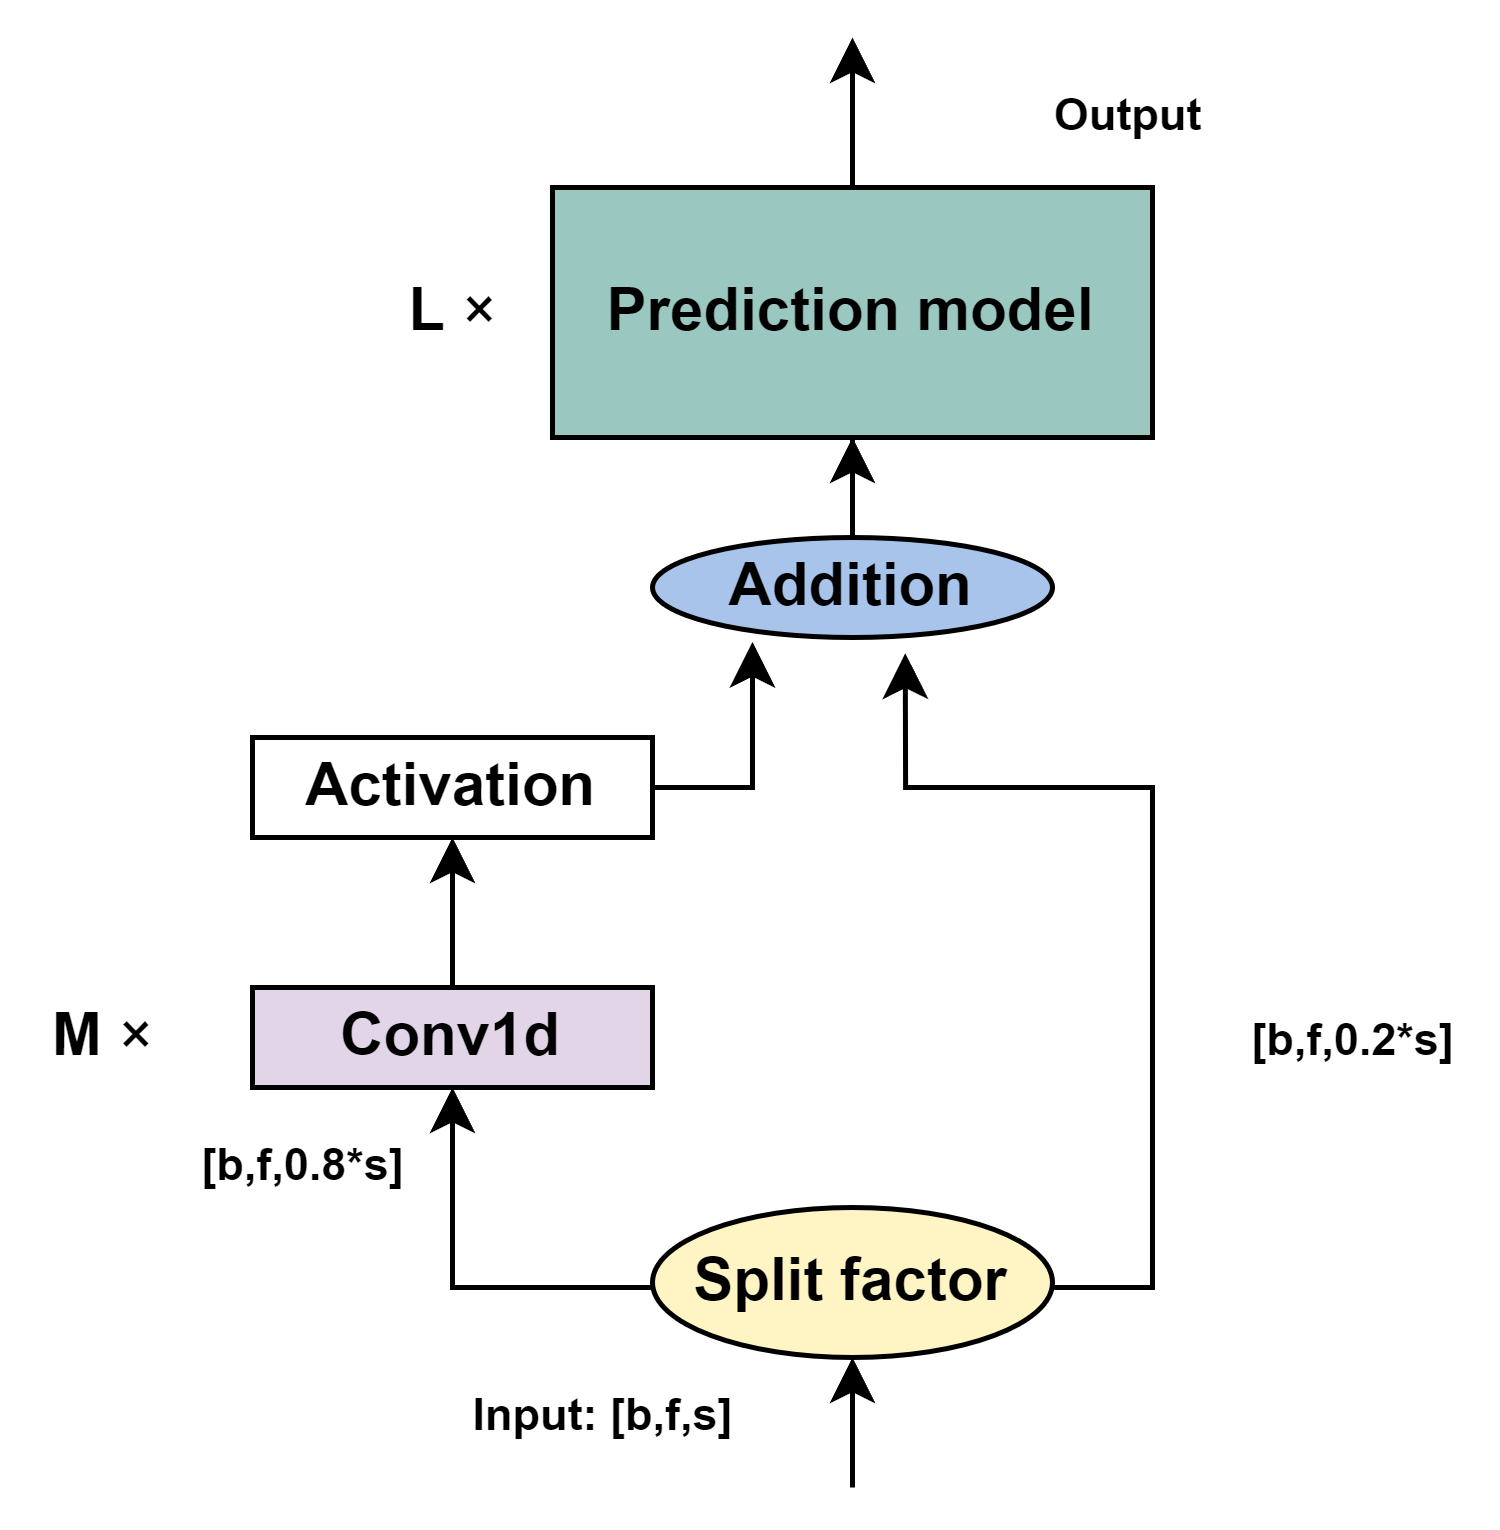
\includegraphics[width=0.8\linewidth]{images/StructureDiagram.drawio.png}
    \caption{Sample TCformer structure}
    \label{fig:Sample TCformer structure}
\end{figure}

The TCformer has a simple and flexible structure. In general, we use CNN for extracting the first $p\%$ of the input data, leaving the rest raw, and feeds it to the prediction model. On fig \ref{fig:Sample TCformer structure}, the split factor is a scalar $p$ that splits the dataset into to on the dimension of sequence length. Note that the split factor is a hyperparameter that needs to be manually assigned. For example, a scalar $p=0.8$ would split the input of shape $X\in \mathbb{R}^{b,f,s}$ into $X\in \mathbb{R}^{b,f,0.8\cdot s}$ and $X\in \mathbb{R}^{b,f,0.2\cdot s}$ where:

\begin{enumerate}
    \item $b$ is the batch size
    \item $f$ is the dimension of feature
    \item $s$ is the sequence length
\end{enumerate}

On fig.\ref{fig:Sample TCformer structure}, there can be $M$ Conv1d layer. They are 1-Dimensional convolution layers that extract traits from the $p\%$ of the input and reduces the sequence length, where $p$ is the split factor and it's set to $0.8$ in this illustration. There could be multiple layers added flexibly. It can be replaced by a Conv2d (needs to ensure that the dimension of the model doesn't reduce). The right branch leaves the raw data that will be joined back with the left branch in the concat component. In concat component the two branches' tensors will be merged on the third dimension $s$. Lastly, the concatenated tensor will be the input for the prediction model. 

\subsection{Convolution extraction}

\begin{figure}[H]
    \caption{Convolutional sequence summary on left branch}
    \centering
    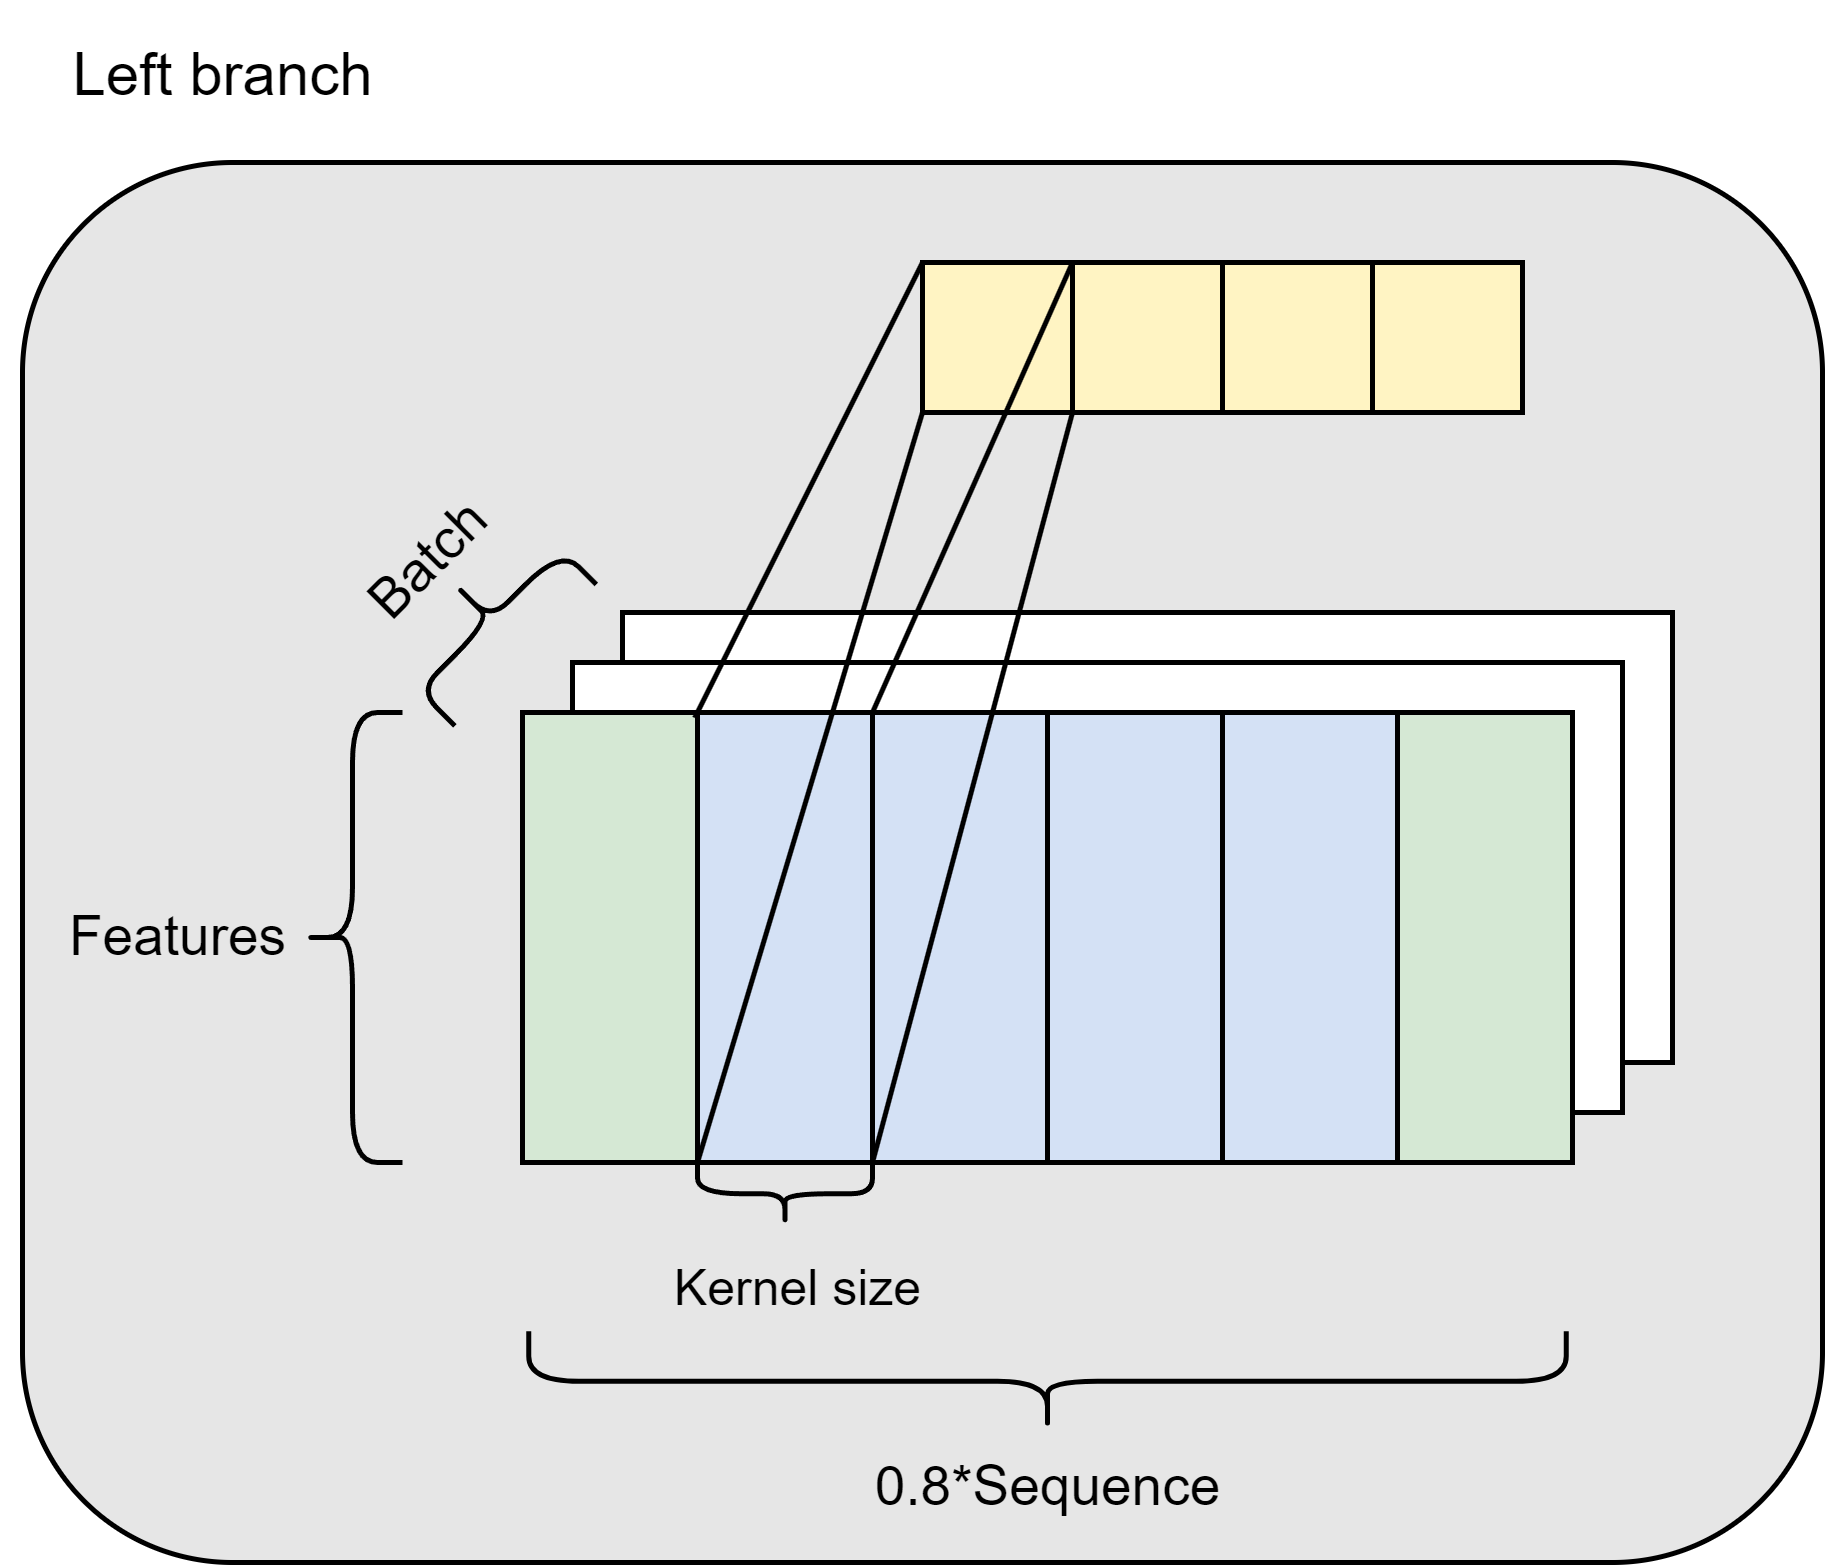
\includegraphics[width=0.7\linewidth]{images/Left branch.png}
    \label{fig:convolutional-operation}
\end{figure}

In the left branch, Conv1d layer is outputting summaries for the first $80\%$ of earlier data, leaving the rest $20\%$ raw for the Transformer encoder to process. This will cause the input $X$ to change it's third dimension's shape $s$ from:

\begin{gather}
    s_1=0.8\cdot s\\
    s_2=\lfloor\frac{0.8\cdot s-k}{r} \rfloor+1
\end{gather}

\begin{enumerate}
    \item $s_1$ is the sequence length before convolution layer
    \item $k$ is kernel size
    \item $s_2$ is the sequence length after convolution layer
    \item $r$ is the stride
\end{enumerate}

On the right branch, the raw data is not processed. Given that the Transformer has already have a good performance on raw data, applying convolution is not needed and might reduce the information perceived in the encoder block. 

\subsection{Parameter reduction}

After the addition, the input for the encoder block will have a sequence length of:

\begin{gather}
    s_3=s_2+0.2\cdot s\\
    =\lfloor\frac{0.8\cdot s-k}{r} \rfloor+1+0.2\cdot s
\end{gather}

The reduction of sequence length $s_3$ compared to $s$ can be calculated:

\begin{gather}
    l=s-s_3\\
    =s-\lfloor\frac{0.8\cdot s-k}{r} \rfloor-1-0.2\cdot s
\end{gather}

Notice $l$ is positively related with $k$ and $r$, changing the stride and kernel size can give a flexible control on the model size. In the attention block, a reduction of $l$ will reduce:

\begin{gather}
    l\times b\times f
\end{gather}

in each of the $Q,K,V$ matrices, largely reducing it's parameters.

\section{Experiments}

We had conducted experiments on 3 real world datasets in the experiment, including weather used in Autoformer \parencite{autoformer} and AMD stock data. 

\subsection{Dataset}

The weather dataset included 52696 rows of data with 21 covariates. 

The AMD stock dataset is accessed through Baostock API \parencite{baostock}. It includes 10995 rows of data with 5 covariates. The data spans from 2nd of January 1981 to 14th of August 2024. 

\subsection{Experiment setup}

Transformer model has a hidden dimension of 8, 2 layers, 2 heads for attention. For all models the optimizer uses Adam, with lr=1e-3, wd=1e-4, dropout=0.1, training in 5 epochs with batch size of 512 with train test $9:1$ splitting. The TCformer uses split factor of 0.8 with the CNN using kernel size 6 with a stride of 6. The criteria uses MSE (Mean Squared Error). 

\subsection{Results}

\begin{table}[H]
\caption{AMD stock data test MSE loss}
\centering
\label{tab:AMD-loss}
\begin{tabular}{rrrr}
\toprule
TCformer1d & transformer & seq\_len & pct\_improve(\%) \\
\midrule
0.018490 & 0.073744 & 16 & 74.93 \\
0.015125 & 0.061805 & 32 & 75.53 \\
0.012830 & 0.053022 & 64 & 75.80 \\
0.017049 & 0.069303 & 128 & 75.40 \\
0.016919 & 0.070958 & 256 & 76.16 \\
0.017332 & 0.072824 & 512 & 76.20 \\
\bottomrule \\
\end{tabular}
\label{tab:comparison}
\end{table}

In table \ref{tab:AMD-loss}, for AMD stock data, the TCformer with 1d in average has improved performance by about 75\%, while having reduced size of model. During experiment, the TCformer was successfully trained on dataset when sequence length is 1024 however the Transformer model failed due to GPU memory overflow, so the sequence length for the experiment is limited up to $512$.

\begin{figure}[H]
    \centering
    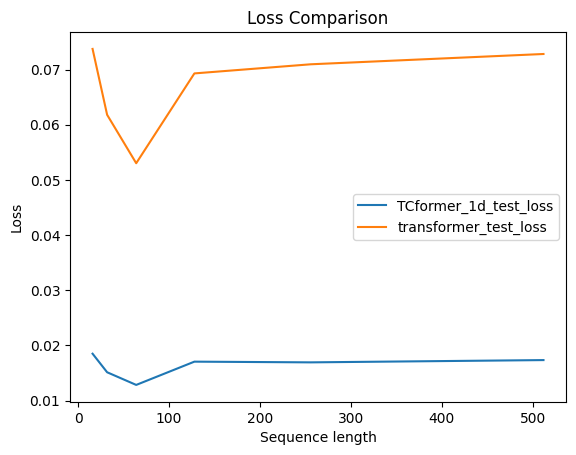
\includegraphics[width=0.8\linewidth]{images/AMD-loss-cmp.png}
    \caption{AMD loss curve}
    \label{fig:AMD-loss-curve}
\end{figure}

On fig.\ref{fig:AMD-loss-curve}, the test loss for both models both has it's minimum at a sequence length of 64. For every sequence length, TCformer has a much lower lost compared to Transformer. The Trasfomer loss shows an increase as sequence length increases from 128 to 512 while this is relatively not as significant in TCformer's loss. This shows that the sequence reduction has enabled TCformer to handle longer sequence while remaining similar precision. 

\begin{table}[H]
\caption{Weather data test MSE loss}
\centering
\label{tab:weather-loss}
\begin{tabular}{rrrr}
\toprule
TCformer1d & transformer & seq\_len & pct\_improve (\%) \\
\midrule
0.026144 & 0.104435 & 16 & 74.97 \\
0.026144 & 0.104253 & 32 & 74.92 \\
0.026188 & 0.103928 & 64 & 74.80 \\
0.025542 & 0.101652 & 128 & 74.87 \\
0.028019 & 0.107837 & 256 & 74.02 \\
0.026371 & 0.104923 & 512 & 74.87 \\
\bottomrule\\
\end{tabular}
\label{tab:comparison}
\end{table}

Like the results in \ref{tab:AMD-loss} 


\begin{figure}[H]
    \centering
    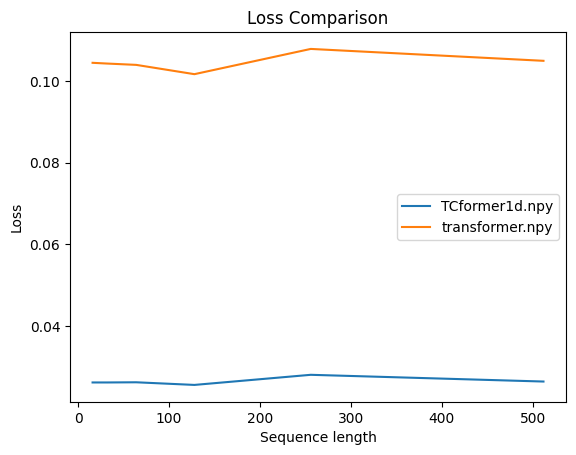
\includegraphics[width=0.8\linewidth]{images/weather-loss-cmp.png}
    \caption{Weather loss curve}
    \label{fig:weather-loss-curve}
\end{figure}

Similar to the results from 

% \appendices
% \section{Appendix title}
% Appendix one text goes here.

% \section{Appendix title}
% Appendix two text goes here.

\section{Conclusion}
The TCformer architecture overall is successful in addressing the limitations of both pure convolutional and transformer models. By integrating temporal convolution with transformer-based attention, TCformer achieves superior predictive performance while maintaining computational efficiency. The model's ability to handle longer sequences and its consistent performance improvements across different datasets suggest its potential for wide applicability in various time series prediction tasks. Future work could explore the model's performance on a broader range of datasets and investigate further optimizations to enhance its efficiency and scalability.


\printbibliography

\end{document}

